\documentclass[12pt]{article}

\usepackage{hyperref} % for auto-linking table of contents
\usepackage{amsmath}
\usepackage[margin=1in]{geometry}
\usepackage{fancyvrb} % fancy verbatim
\usepackage{fancyhdr}
\usepackage{graphicx}
\usepackage{float}
\usepackage{tikz} % for \foreach
\usepackage{caption}
\usepackage{subcaption}

\usepackage{paralist}
\usepackage{listings}
\usepackage{color}

\definecolor{dkgreen}{rgb}{0,0.6,0}
\definecolor{gray}{rgb}{0.5,0.5,0.5}
\definecolor{mauve}{rgb}{0.58,0,0.82}

\lstset{frame=tb,
  language=Matlab,
  aboveskip=3mm,
  belowskip=3mm,
  showstringspaces=false,
  columns=flexible,
  basicstyle={\small\ttfamily},
  numbers=none,
  numberstyle=\tiny\color{gray},
  keywordstyle=\color{blue},
  commentstyle=\color{dkgreen},
  stringstyle=\color{mauve},
  breaklines=true,
  breakatwhitespace=true
  tabsize=3
}


\hypersetup{
    bookmarks=true,         % show bookmarks bar?
    unicode=false,          % non-Latin characters in Acrobat�s bookmarks
    pdftoolbar=true,        % show Acrobat�s toolbar?
    pdfmenubar=true,        % show Acrobat�s menu?
    pdffitwindow=false,     % window fit to page when opened
    pdfstartview={FitH},    % fits the width of the page to the window
    pdftitle={My title},    % title
    pdfauthor={Author},     % author
    pdfsubject={Subject},   % subject of the document
    pdfcreator={Creator},   % creator of the document
    pdfproducer={Producer}, % producer of the document
    pdfkeywords={keyword1} {key2} {key3}, % list of keywords
    pdfnewwindow=true,      % links in new PDF window
    colorlinks=true,       % false: boxed links; true: colored links
    linkcolor=blue,          % color of internal links (change box color with linkbordercolor)
    citecolor=green,        % color of links to bibliography
    filecolor=magenta,      % color of file links
    urlcolor=cyan           % color of external links
}

\pagestyle{fancy}
\lhead{Daniel McArdle}
\chead{Homework 2}
\rhead{CSE 573: Computer Vision}
\cfoot{\thepage}


\begin{document}

\title{Homework 2: Segmentation}
\author{Daniel McArdle\\
CSE 573: Computer Vision}
\date{October 24, 2014}
\maketitle  % without this line, the header would not be generated

% \tableofcontents

\section{Implementation}

My implementation of \texttt{segmentImg} begins by using the given \texttt{makeLMfilters} function to create the LM filter bank.  For each filter, we save the response as a layer in a 3D matrix. Next, we compute the \texttt{X} matrix, which has \texttt{rows*cols} rows and \texttt{num\_filters} columns.  In other words, each pixel has a column and each row entry represents the filter response for that pixel.

Next, we perform K-Means Clustering on the \texttt{X} matrix.  \textit{Note: I implemented my own K-Means Clustering algorithm.} Initially, my implementation was very slow because, for each point, we were finding the closest center with a nested loop.  I was able to greatly improve the speed by using \href{http://www.mathworks.com/help/stats/knnsearch.html?refresh=true}{knnsearch}, a function from the Statistics toolbox.

There are a number of problems with the output of this implementation.  The biggest issue is that the segmented regions have many holes in them.  For example, the cheetah has some large holes in its face.  This could be because the K-Means Clustering algorithm does not take spatial proximity into account, only similarity of filter responses.


\section{Results}

\subsection{Segmented Animals}

\begin{figure}[H]
	\begin{subfigure}[b]{0.48\textwidth}
        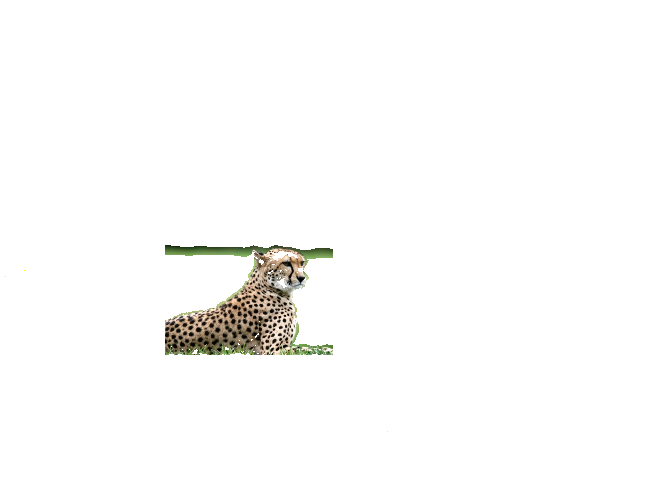
\includegraphics[width=\textwidth]{../output/cheetah4.png}
        \caption{Cheetah Segmentation with $k=8$}
        \label{fig:CheetahSeg}
	\end{subfigure}
	\begin{subfigure}[b]{0.48\textwidth}
        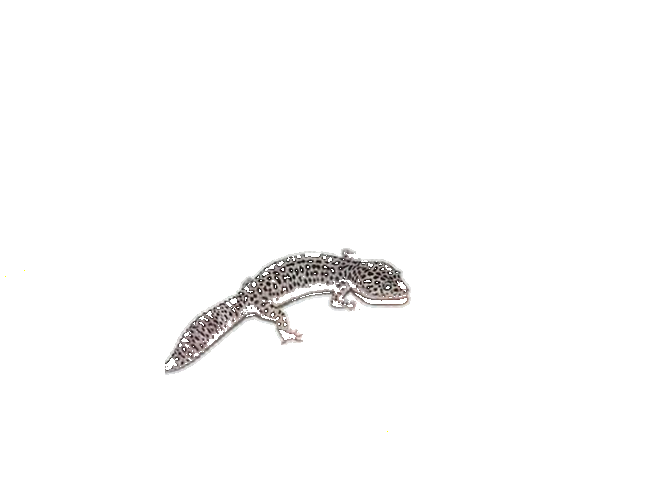
\includegraphics[width=\textwidth]{../output/gecko4.png}
        \caption{Gecko Segmentation with $k=6$}
        \label{fig:DogSeg}
	\end{subfigure}
\end{figure}

\subsection{Transferred Foregrounds}

\begin{figure}[H]
	\begin{subfigure}[b]{0.9\textwidth}
        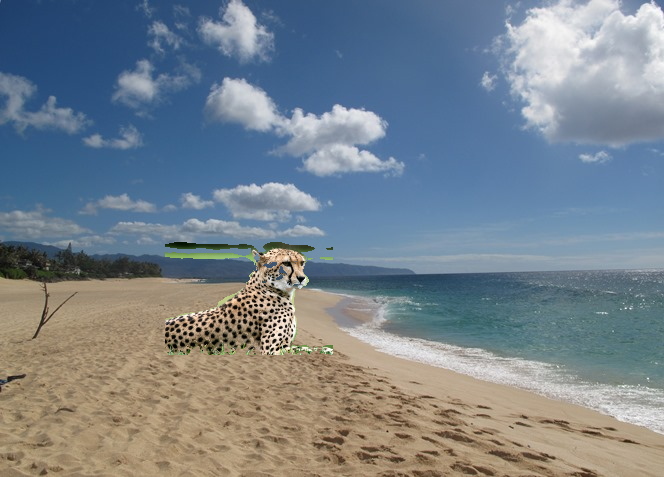
\includegraphics[width=\textwidth]{../output/cheetah1.png}
        \caption{Cheetah}
        \label{fig:Cheetah}
	\end{subfigure}
	
	\begin{subfigure}[b]{0.9\textwidth}
        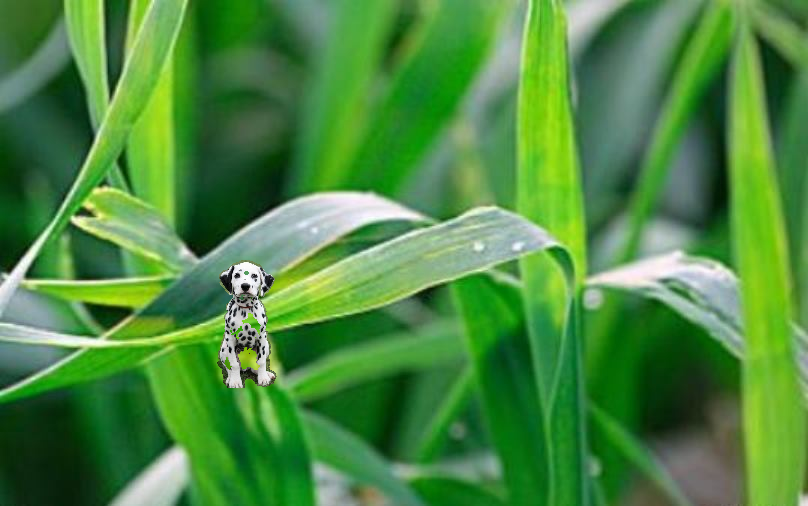
\includegraphics[width=\textwidth]{../output/dog22.png}
        \caption{Dog}
        \label{fig:Dog}
	\end{subfigure}

	\begin{subfigure}[b]{0.9\textwidth}
        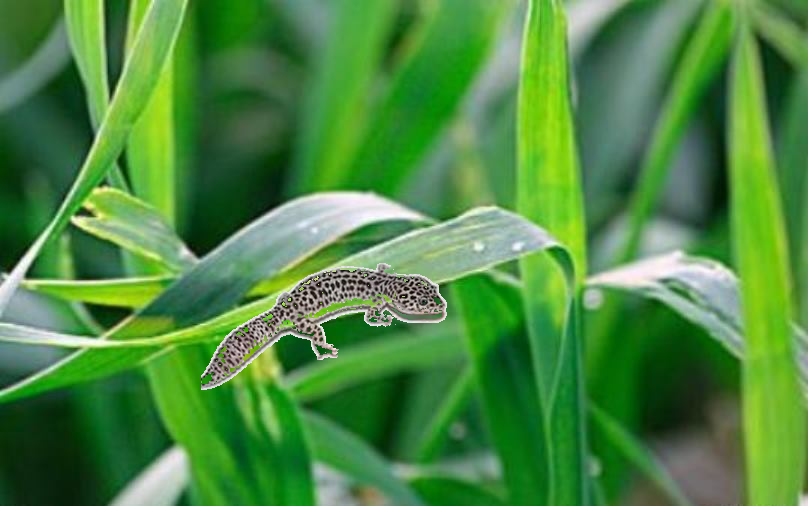
\includegraphics[width=\textwidth]{../output/gecko2_k=5.png}
        \caption{Gecko}
        \label{fig:Gecko}
	\end{subfigure}
	
	\begin{subfigure}[b]{0.9\textwidth}
        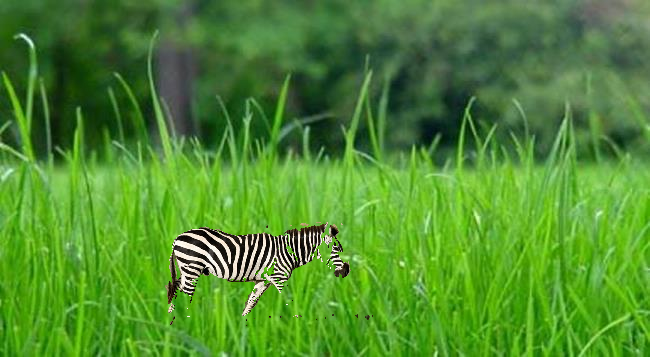
\includegraphics[width=\textwidth]{../output/zebra3_k=4.png}
        \caption{Zebra}
        \label{fig:Zebra}
	\end{subfigure}
\end{figure}



\end{document}
